%\iffalse
\let\negmedspace\undefined
\let\negthickspace\undefined
\documentclass[journal,12pt,twocolumn]{IEEEtran}
\usepackage{cite}
\usepackage{amsmath,amssymb,amsfonts,amsthm}
\usepackage{algorithmic}
\usepackage{graphicx}
\usepackage{textcomp}
\usepackage{xcolor}
\usepackage{txfonts}
\usepackage{listings}
\usepackage{enumitem}
\usepackage{mathtools}
\usepackage{gensymb}
\usepackage{comment}
\usepackage[breaklinks=true]{hyperref}
\usepackage{tkz-euclide} 
\usepackage{listings}
\usepackage{gvv}                                        
\def\inputGnumericTable{}                                 
\usepackage[latin1]{inputenc}                                
\usepackage{color}                                            
\usepackage{array}                                            
\usepackage{longtable}                                       
\usepackage{calc}                                             
\usepackage{multirow}                                         
\usepackage{hhline}                                           
\usepackage{ifthen}                                           
\usepackage{lscape}

\newtheorem{theorem}{Theorem}[section]
\newtheorem{problem}{Problem}
\newtheorem{proposition}{Proposition}[section]
\newtheorem{lemma}{Lemma}[section]
\newtheorem{corollary}[theorem]{Corollary}
\newtheorem{example}{Example}[section]
\newtheorem{definition}[problem]{Definition}
\newcommand{\BEQA}{\begin{eqnarray}}
\newcommand{\EEQA}{\end{eqnarray}}
\newcommand{\define}{\stackrel{\triangle}{=}}
\theoremstyle{remark}
\newtheorem{rem}{Remark}
\begin{document}
\bibliographystyle{IEEEtran}
\vspace{3cm}
\title{\textbf{11.9.3.7}}
\author{EE23BTECH11210-Dhyana Teja Machineni$^{*}$% <-this % stops a space
}
\maketitle
\newpage
\bigskip

\section*{Exercise 9.3}
7. \hspace{2pt}Find the sum to indicated number of terms in each of the geometric progressions in
$$0.15, 0.015, 0.0015\ldots 20 terms$$.

\solution
\begin{flushleft}
     \begin{table}[h]
         \label{tab:table2}
         \caption{Variables and their descriptions}
         \renewcommand{\arraystretch}{1.5}
\begin{tabular}{|c|c|c|}
\hline
Parameter & Description & Value \\\hline
\( n \) & No. of terms in the G.P &20 \\\hline
\(x(0) \) & first term in the G.P&0.15 \\\hline
\( r \) & common ratio in the G.P& 0.1 \\\hline
\( x(n) \) & nth term in the G.P& none \\\hline
\( X(z) \) & Z transform of x(n)& none \\\hline
\( Y(z) \) & Z transform of y(n)& none \\\hline
\(y(n)\)& Sum of n terms of GP& none\\\hline
\end{tabular}

     \end{table}
 \end{flushleft}
\begin{align}
x(n) &= x(0)r^n \\
X(z) &= \frac{x(0)}{1-rz^{-1}} \qquad |z| > |r| \\
U(z)&=\frac{1}{1-z^{-1}}, \qquad |z|>1\\
y(n)&= x(n)*u(n)\\
Y(z)&=X(z)U(z)\\
&=\left\{ \frac{0.15}{1-0.1z^{-1}}\right\}\left\{\frac{1}{1-z^{-1}}\right\}\quad|z| > 1\quad|z|>|0.1|
\end{align}
Use Counter integration to find the inverse of the z transform which gives sum of n terms
\begin{align}
y(20)&=\frac{1}{2\pi j}\oint_C \frac{0.15 z^2}{(z-1)(z-0.1)}z^{19} dz\\
&=\frac{1}{2 \pi j}\oint_C \frac{0.15}{0.9} \left\{\frac{1}{z-1} - \frac{1}{z-0.1} \right\}z^{21}dz\\
&= \frac{1}{6} \left\{\left\{\lim_{z\to \ 1}\frac{z^{21}}{z-1} (z-1) \right\}-\left\{\lim_{z \to \ 0.1}\frac{z^{21}}{z-0.1} (z-0.1)\right\}\right\}\\
&= \frac{1}{6}(1- 0.1^{21})\\
    &=0.16667
\end{align}
        $\therefore$ Sum of $20$ terms of the given GP is $0.16667$
       \renewcommand{\thefigure}{\theenumi}
 \renewcommand{\thetable}{\theenumi}
\begin{figure}[h]
  
  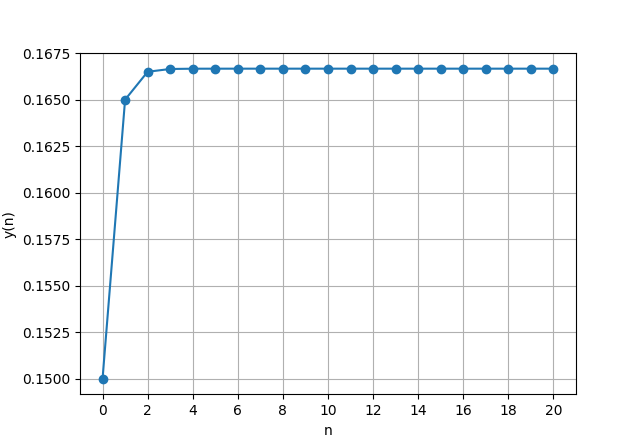
\includegraphics[width=1.0\columnwidth]{figs/graph.png}
  \caption{Stem plot of y(n)}
  \label{fig:your_label}
\end{figure}


\end{document}
